\chapter{Division implementation}\label{Chapter_Impl_Div}
\section{Introduction}
The purpose of this chapter is to introduce and explain the hardware implementation of the Radix-4 SRT division algorithm using the \textit{minimally redundant digit set}.
The algorithm will first be presented in the form of high-level code and only some information about the operations to be performed will be given: the detailed explanation of all the assumptions and the reason why some operations are performed can be found in \autoref{Chapter_SRT}.

The starting point of the circuit is the algorithm to be implemented, and its code is presented in \autoref{code:srt_radix4}.
The division circuit is split into two sub-units: a controller which keeps track of what operation should be performed  and a datapath which actually performs the necessary operations.

\begin{lstlisting}[label={code:srt_radix4}, caption={The C++ code implementing the Radix-4 SRT division}, language=C++]
std::pair<SLV::std_logic_vector, SLV::std_logic_vector> 
Division::srt_division_radix_4_digit_2
(SLV::std_logic_vector& dividend, SLV::std_logic_vector & divisor){

    // PREPROCESSING
    int N = dividend.size;

    // Also detects divide by zero operation
    if(dividend.to_base_10() >= (divisor.to_base_10() << N/2)
        throw std::invalid_argument("Can't compute with these values");
 
    // Temporary reminder
    SLV::std_logic_vector A (N   + 3);
    // Divisor
    SLV::std_logic_vector B (N/2 + 2);
    // Quotient
    SLV::std_logic_vector Q (N/2 + 2);

    // Leading zeros of the divisor
    unsigned int k = divisor.extract(N/2 - 1, 0).count_leading_zeros();

    A = SLV::std_logic_vector("000") & (dividend << k);
    // Since the divisor and the dividend are both N long, the real divisor is in the 
    // bottom part of "divisor"
    B = SLV::std_logic_vector("00") & (divisor.extract(N/2 - 1, 0) << k);

    // DIVISION
    for(int i = 0; i <= (N/2 >> 1) ; i++){
        SLV::std_logic_vector A_upper  = A.extract(N + 1, N/2);
        SLV::std_logic_vector A_bottom = A.extract(N/2 - 1, 0);

        SLV::std_logic_vector partial_R(N/2 + 2);

        int current_q = srt_division_radix_4_lut_digit_2(
            B.extract(N/2 - 2, N/2 - 4) & 
            A.extract(N + 2, N - 3)
        );

        if(current_q == 2){
            Q = (Q << 2) + 2;
            partial_R = A_upper - (B << 1);
        }
        if(current_q == 1){
            Q = (Q << 2) + 1;
            partial_R = A_upper - B;
        }
        if(current_q == 0){
            Q = Q << 2;
            partial_R = A_upper;
        }
        if(current_q == -1){
            Q = (Q << 2) - 1;
            partial_R = A_upper + B;
        }
        if(current_q == -2){
            Q = (Q << 2) - 2;
            partial_R = A_upper + (B << 1);
        }
        
        A = (SLV::std_logic_vector("0") & partial_R & A_bottom) << 2;
    }

    // SIGN CORRECTION
    if(A.get_msb() == 1){
        Q = Q - 1;
        A = (SLV::std_logic_vector("0") & 
             ((SLV::std_logic_vector("0") & A.extract(N + 2, N/2 + 2)) + B) 
             & A.extract(N/2 + 1, 2) ) << 2;
    }
    
    Q = Q.extract(N/2 - 1, 0);
    SLV::std_logic_vector R = A.extract(N + 1, N/2 + 2) >> k;

    return std::pair<SLV::std_logic_vector, SLV::std_logic_vector>
    (Q, R);
}
\end{lstlisting}

\section{Controller}\label{sect:srt_controller}
The basic operations to be performed are:
\begin{enumerate}
    \item Preprocess the dividend and the divisor;
    \item Divide;
    \item Correct the quotient and the remainder, if necessary;
    \item Postprocess the quotient and the result.
\end{enumerate}
The details of these procedures are given in \autoref{sect:srt_datapath}. 

The controller has one state for each activity plus the \texttt{idle} state, and a simplified state diagram (most of the control signals are omitted for brevity) is in \autoref{fig:controller_state_diagram}. 
It's important to know that $N$ represents the length of the \textbf{dividend}, which in AFTAB is the width of a register, so 32 bits.
\begin{figure}
    \centering
    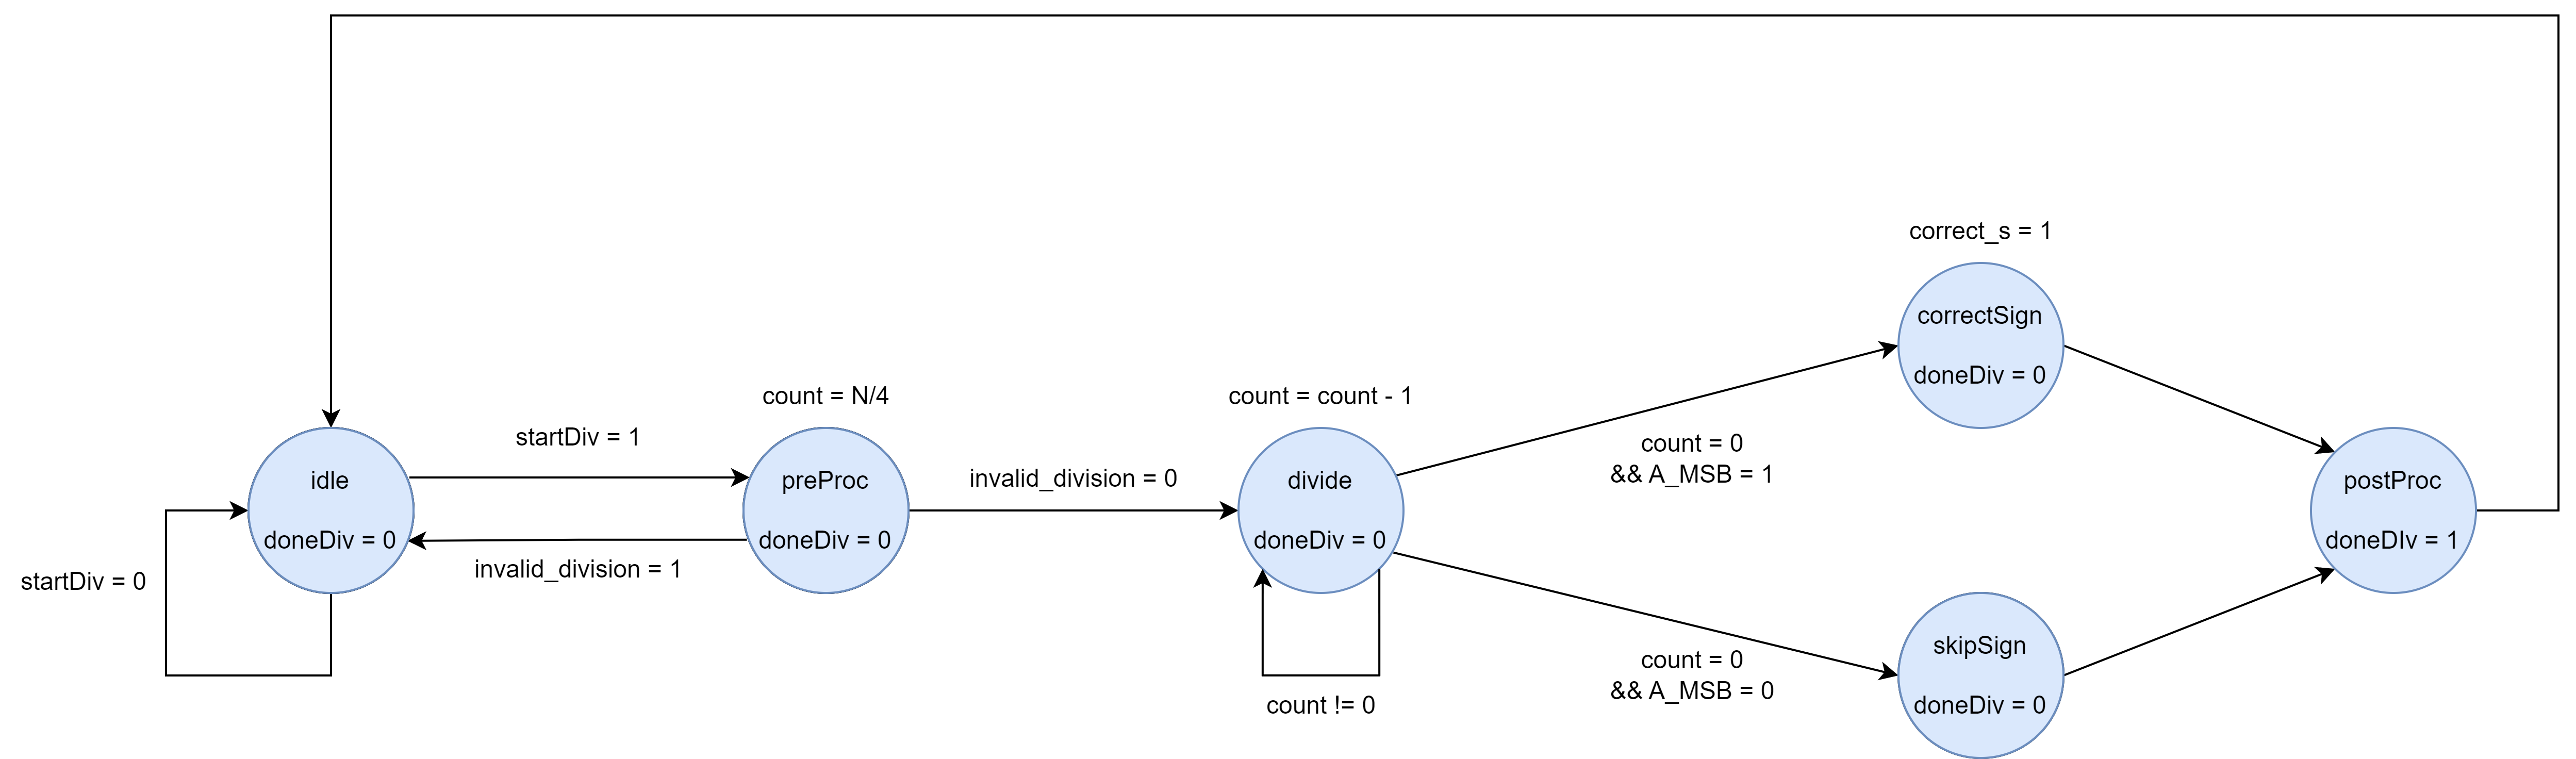
\includegraphics[width=150mm]{images/SRTControllerStateDiagramSimplified.png}
    \caption{Simplified sate diagram of the controller}
    \label{fig:controller_state_diagram}
\end{figure}
Upon reset, the controller is initialised to the \texttt{idle} state and waits for the processor's control unit to assert the \texttt{startDiv} signal, thus requesting a division to be performed.

After that, the controller moves into the \texttt{preProc} state and asserts the control signals to perform the preprocessing of the operands.

The next state depends on the \texttt{invalid\_division} signal, which is generated by the datapath and represents, as the name implies, whether the division is valid or not due to the values of dividend and divisor (which also includes the case of a division by 0).
Assuming the division is feasible, the controller moves to the \texttt{divide} state: here the quotient and remainder are iteratively calculated.
Since two digits of the quotient are computed per clock cycle and the quotient is $N / 2 = 16 \text{ bits}$ long, the controller stays in this state for 8 clock cycles.

After all the iterations of the division have been performed, the controller's next state depends on the remainder's sign: if it's negative both the quotient and the remainder itself need to be corrected, so the controller moves to the \texttt{correctSign} state and asserts some signals to instruct the datapath to perform the sign-correction operations.
If the remainder is not negative then the quotient and remainder are correct, so the division is concluded, and all that is missing is the postprocessing. 
Nonetheless, in this case the controller moves to the \texttt{skipSign} state for consistency: it's undesirable for an operation's execution to take a variable amount of clock cycles depending on its inputs' values.
Thus, to make sure the division has a constant duration in terms of clock cycles, the datapath remains idle while the controller is in the \texttt{skipSign} state.

After the division is completed the operands need to be postprocessed, so regardless of whether the sign correction was performed or not the controller moves to the \texttt{postProc} state. 
In this state that final outputs of the division circuit are made ready to be used by any unit outside of the device and a signal that warns the processor's control unit is asserted.

These results are available for one clock cycle (technically less than one, since postprocessing takes some time), and after that the controller goes back to the \texttt{idle} state and will wait to be instructed to run the division again.

\section{Datapath}\label{sect:srt_datapath}
The datapath is split into a wrapper and the actual division unit: the former is built around the latter because the SRT division requires its operands to be normalised (so preprocessed), and then will produce a quotient and a remainder that will have to be postprocessed to match some characteristics of the original input operands (like signs).

\subsection{Wrapper}
\begin{figure}
    \centering
    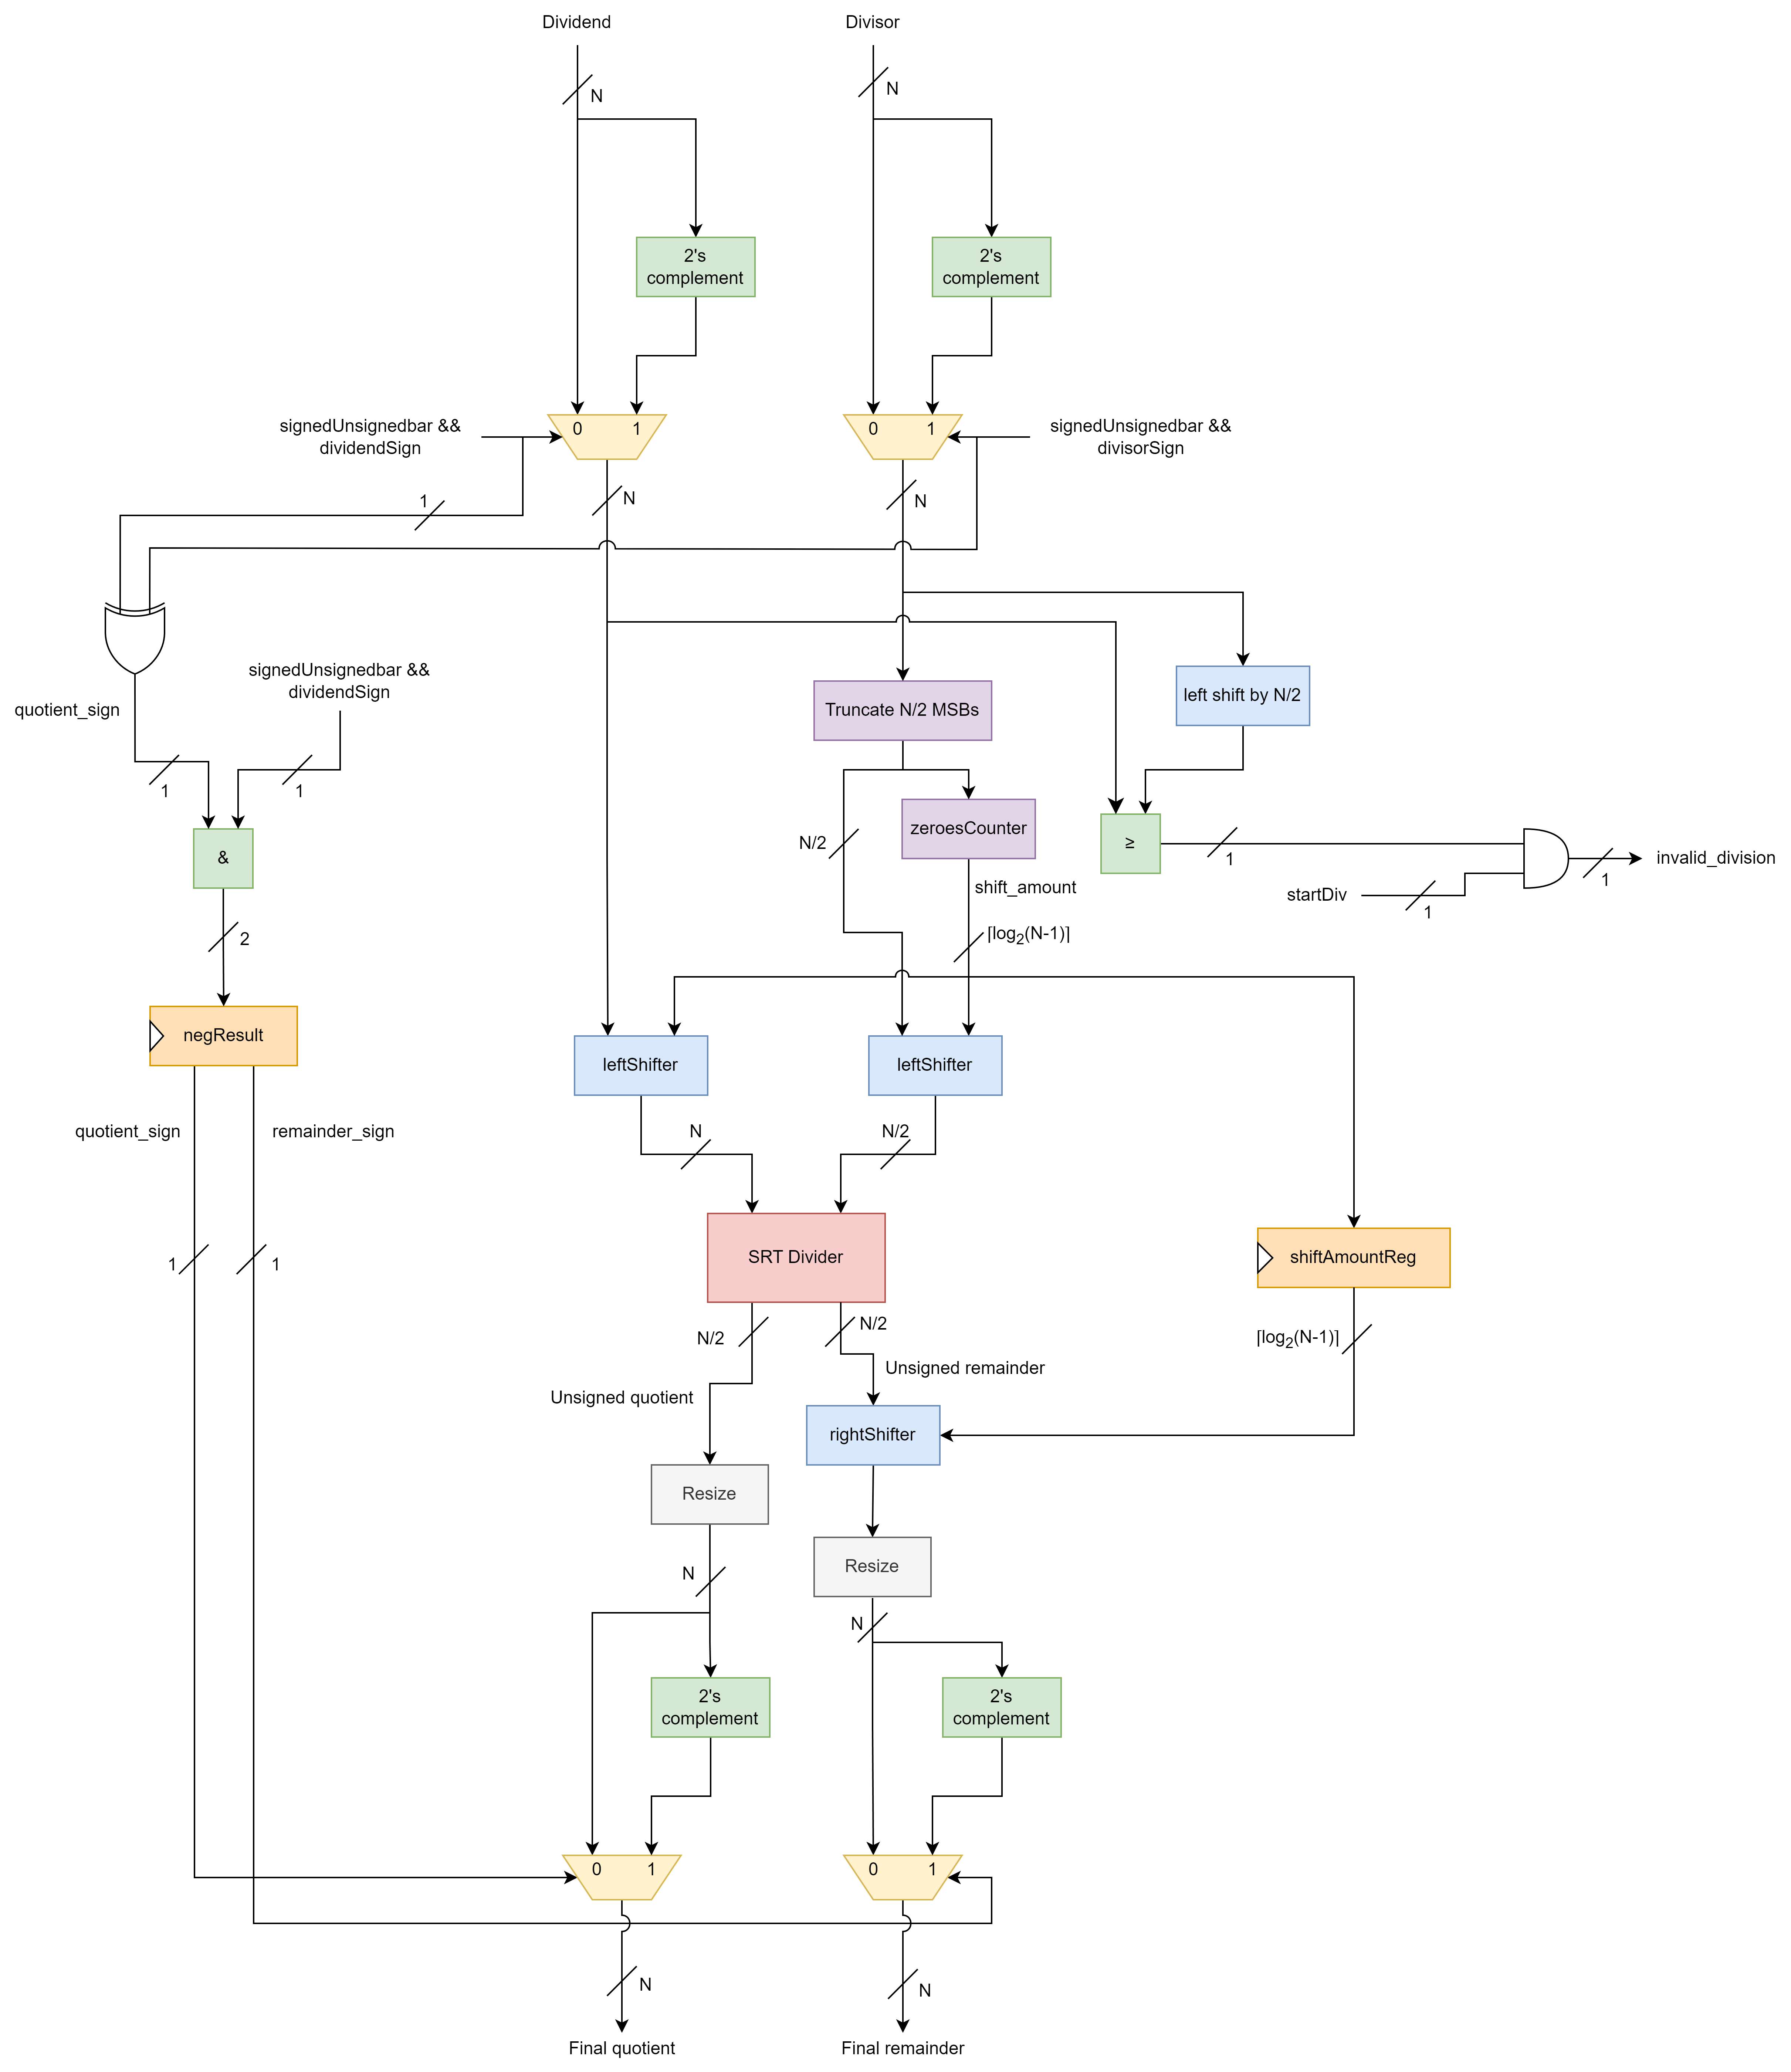
\includegraphics[width=150mm]{images/SRTWrapper.png}
    \caption{Diagram of the wrapper}
    \label{fig:wrapper_diagram}
\end{figure}
The diagram of the wrapper is shown in \autoref{fig:wrapper_diagram} (most control signals are omitted for brevity): all the blocks above the \texttt{SRT Divider} unit are employed in the preprocessing phase, while all the blocks below it are used while postprocessing.
The registers (represented by rectangles with a triangle inside them) are used to persist some information generated during preprocessing that is needed while postprocessing.

\subsubsection{Preprocessing}\label{preprocessing_ch}
The purpose of this phase is to turn the input operands, which can be signed or unsigned integers, into numbers that comply with the assumptions made by the SRT divider: the dividend has to be a 32-bit unsigned number, while the divisor has to be a 16-bit unsigned number with 1 as its MSB.
Before normalising the operands, they need to be converted (if necessary) to unsigned numbers by complementing them.
To do so a copy of the operands is complemented and both the original values and the complemented ones flow into two multiplexers: these select their output depending on whether the division to be performed is between signed operands (\texttt{signedUnsignedBar}, a signal that is controlled by the processor's control unit and that depends on the instruction to be executed, is asserted) and on their inputs' signs (so the MSBs).
Specifically, an operand is considered negative if \texttt{signedUnsignedBar} and its MSB are both 1: in this case its complement is selected; in all other cases the unchanged input goes through the multiplexer because it's either unsigned or signed positive.

After the inputs have been converted to unsigned numbers, the check on the division's validity is performed: if $2^N \cdot divisor \ge dividend$ and a division should be performed (\texttt{startDiv} is asserted), then the division is invalid and the corresponding signal is asserted; this will cause the controller to change state (as previously explained) and the processor's control unit will handle this situation.
In the meantime, in order to normalise the divisor, its $N/2$ MSBs are truncated and a component counts the leading zeroes of the resulting sub-string: this quantity is called \texttt{shift\_amount} and is used by a left-shifter to move the first 1 of the shortened divisor to its MSB.
In order to preserve the ratio between the orders of magnitude of the dividend and the divisor, we also left-shift the dividend by \texttt{shift\_amount}, which is also saved in the register \texttt{shiftAmountReg}: we need to keep this information as we'll need it to compensate for these left-shifts during postprocessing.

We also need to save information about what the sign of quotient and remainder should be once they're calculated, and we need to do this now as only during preprocessing do we have access to the original inputs: the sign of the quotient is the product of the dividend's and divisor's signs (logically speaking it's an XOR), while the sign of the remainder is the same as dividend's.
This information is stored as two bits in the register \texttt{negResult}: its MSB is 1 if the final quotient should be negative and the LSB is 1 if the final remainder should be negative.
Once all the operations explained so far have been executed, the preprocessed operands are passed to the division circuit.

\subsubsection{Postprocessing}
The division circuit will output quotient an remainder as 16-bit unsigned numbers.
In order to restore the ratio between the orders of magnitude of the dividend/divisor and the remainder, the latter first needs to be right-shifted by \texttt{shift\_amount} (which was saved in \texttt{shiftAmountReg}).
The quotient, on the other hand, is of the right order of magnitude and doesn't need to be changed at this time.

After this first operation, both quotient and remainder are resized to match the length of the inputs by simply pushing $N/2$ zeroes as their MSBs, so that the resized numbers are still unsigned and their value is unchanged.

The last step of postprocessing consists in changing the quotient and remainder's sign, if needed. 
The way this operation is performed is similar to the way the dividend's and the divisor's signs were handled: copies of the resized quotient and remainder are complemented, and both the original values and their complements (which are always negative) flow into two multiplexers controlled by the information that was saved in \texttt{negResult}: if the MSB of this register is 1 the quotient has to be negative (its complement is chosen), else the positive quotient is chosen; if the LSB of this register is 1 the remainder has to be negative, else the positive remainder is chosen.

Thus we obtain the final quotient and remainder: they are passed to the processor which will use them as needed.

\subsection{Divider}
The diagram of the divider is shown in \autoref{fig:divider_diagram} (most control signals are not shown for brevity).

\begin{figure}
    \centering
    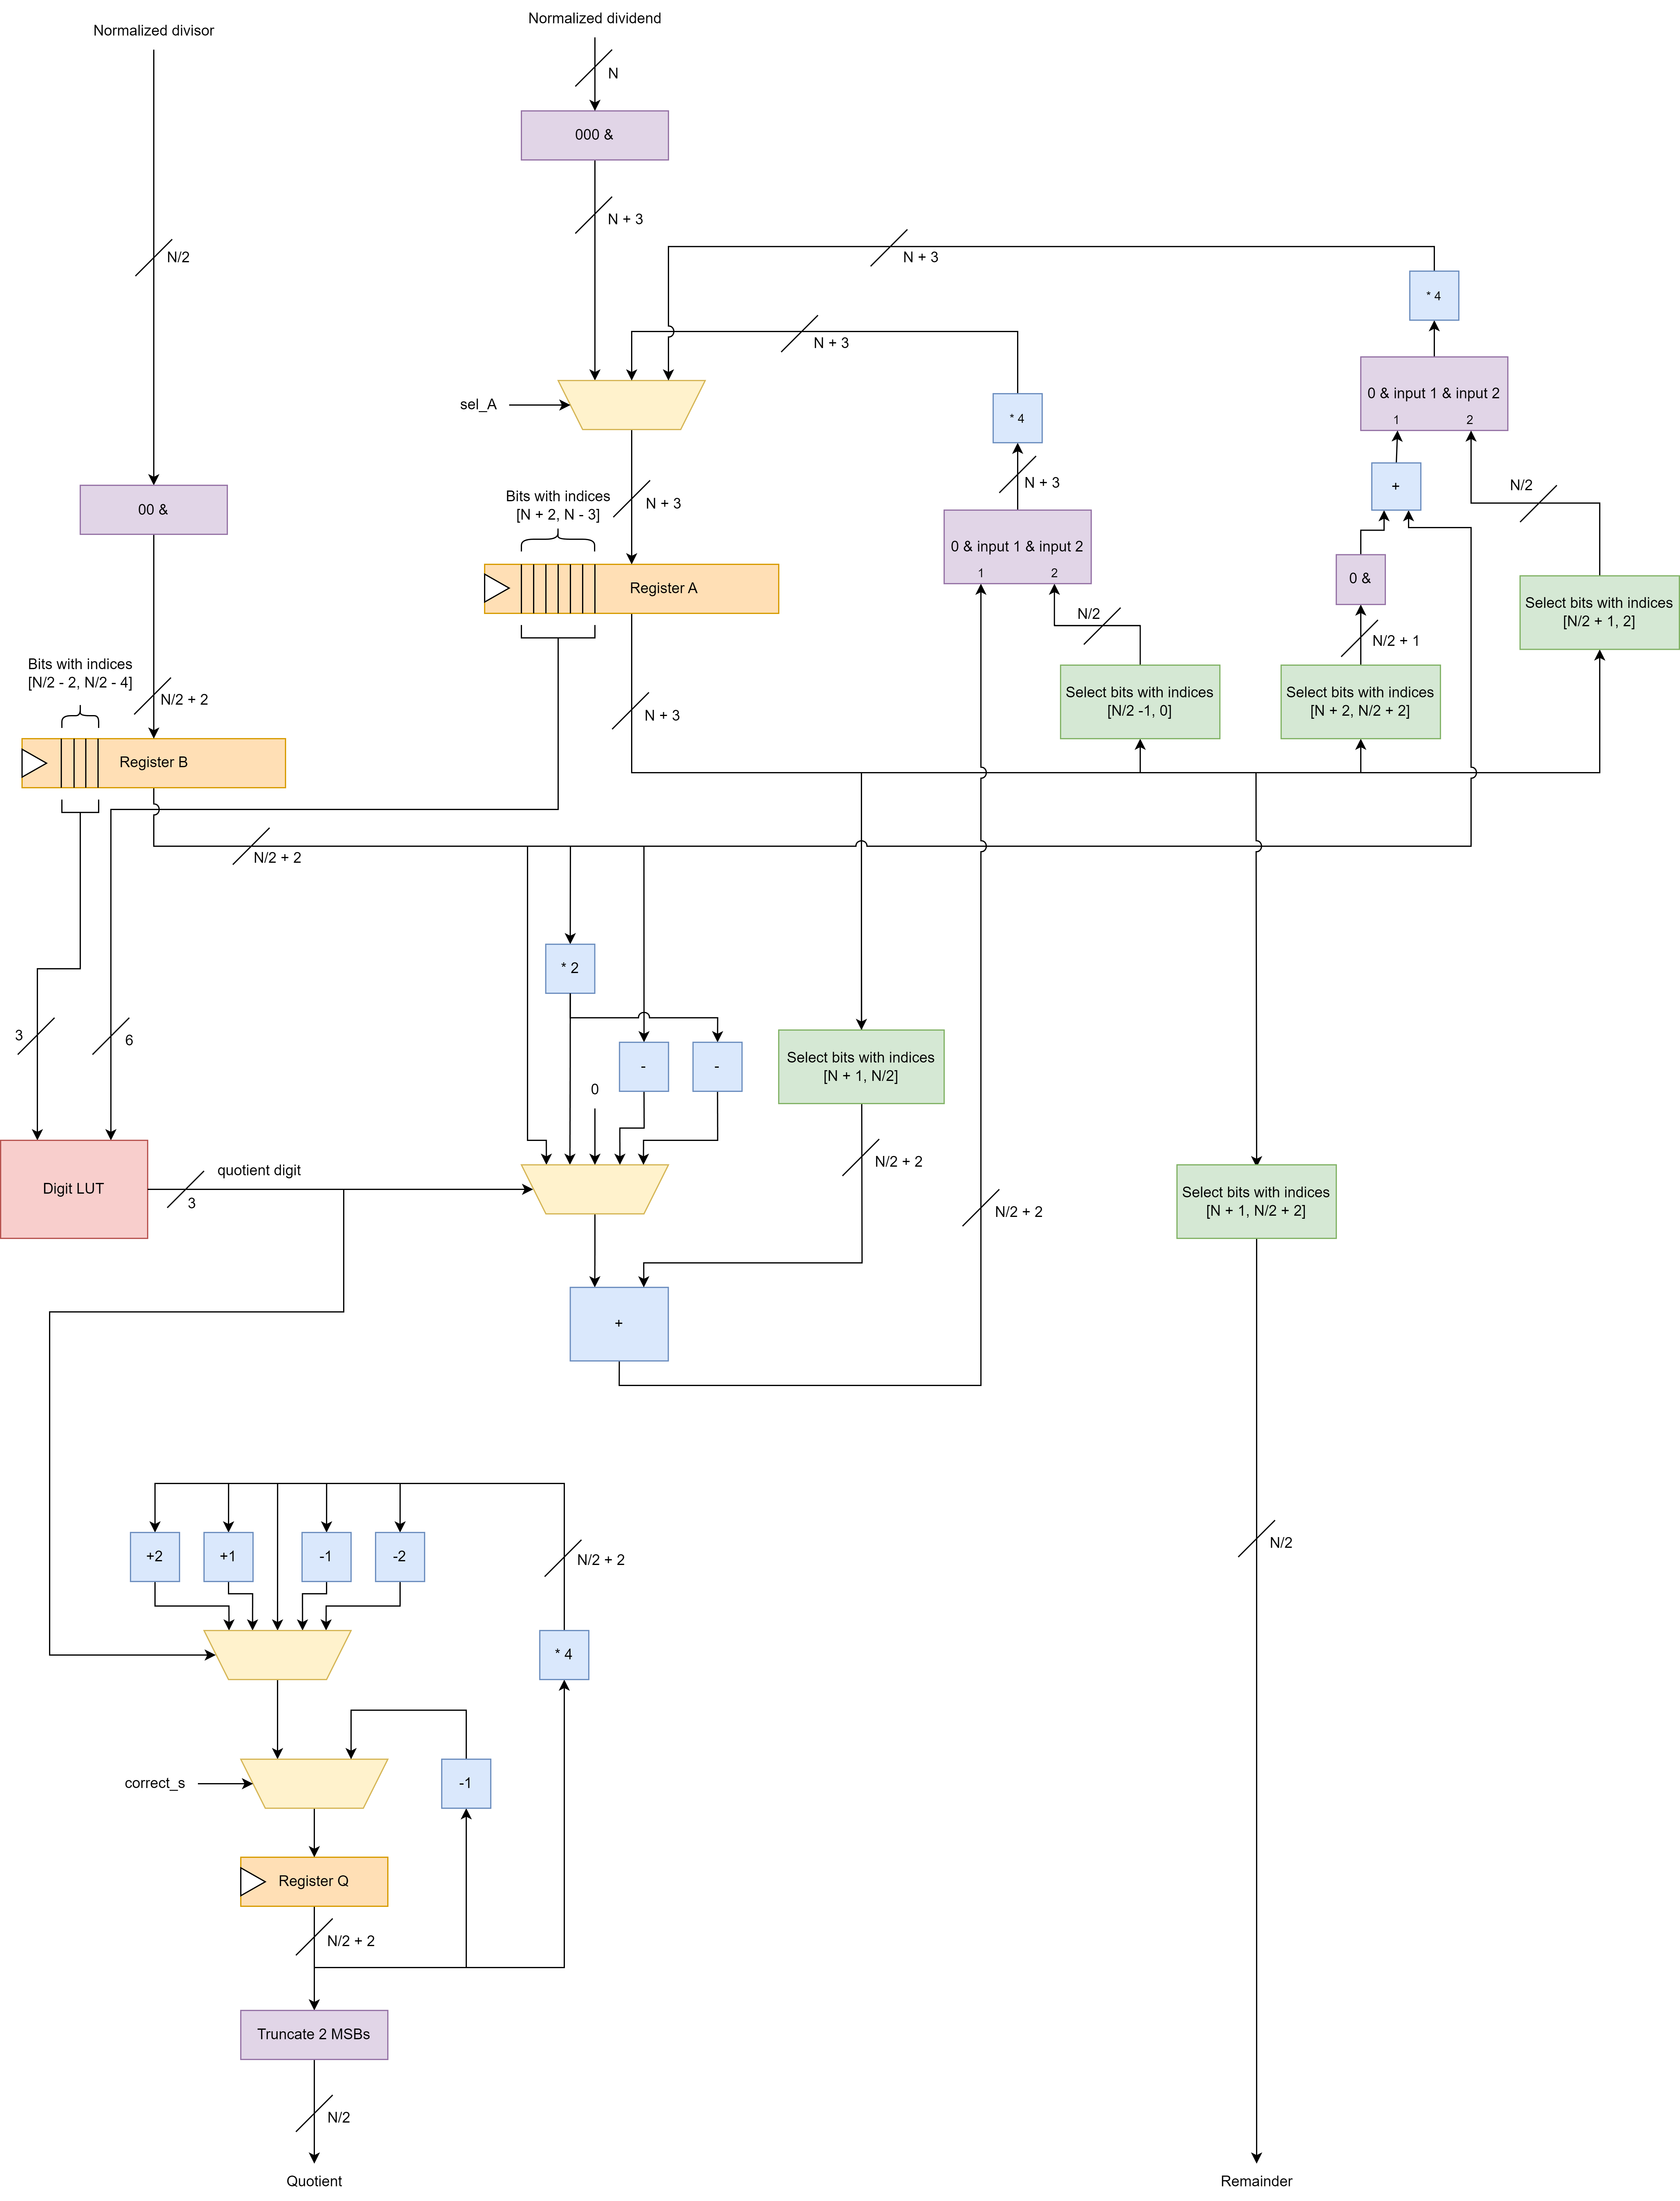
\includegraphics[width=150mm]{images/SRTDivider.png}
    \caption{Diagram of the divider}
    \label{fig:divider_diagram}
\end{figure}

In this component there are three registers (represented as they were in the wrapper): 
\begin{itemize}
    \item \texttt{A} will contain the dividend at first, and then the intermediate remainders while they're calculated;
    \item  \texttt{B} will contain the divisor;  
    \item \texttt{Q} will contain the quotient while it's calculated.
\end{itemize}

Let's begin by analysing register \texttt{B}: its value is only written with the preprocessed divisor after two zeroes have been pushed as its MSB, and this happens when the controller is in the \texttt{preProc} state.

Register \texttt{Q}'s value is initialised to zero before each division, and it's iteratively computed by adding $\pm 1$, $\pm 2$ or $0$ to its current value left-shifted by 2.
The aforementioned numbers are the digits computed during the current iteration of the division and are generated by the \texttt{digit LUT} component, which is a memory implementing the digit selection table as shown in \autoref{tab:srt_radix4}.
The address used to access this memory is obtained by concatenating register \texttt{B}'s bits with indices in the range $ [ N/2 - 2, N/2 - 4 ]$ with register \texttt{A}'s bits with indices in the range $ [ N + 2, N - 3 ]$.
This means that this address is 9 bits wide and that the memory is made of 512 cells.
If the correction of the remainder's sign is needed at the end of the division (so the \texttt{correct\_s} signal is asserted), \texttt{Q}'s value is decremented by 1.
Its value is finally provided to the wrapper after the two MSBs are truncated.

\texttt{A}'s handling, on the other hand, is more complex: its next value depends on both the controller, which will choose which operation should be performed by using the \texttt{sel\_A} signal, and on the quotient digit $q$ that has been calculated during the current iteration.
The possible operations to be performed depend on the controller's state:
\begin{itemize}
    \item when \texttt{sel\_A} is \enquote{00} the controller is in the \texttt{preProc} state, so the preprocessed divisor is saved into \texttt{A} after three zeroes are pushed as its MSB;
    \item when \texttt{sel\_A} is \enquote{01} the controller is in the \texttt{divide} state, so \texttt{A} is loaded with the value of the next intermediate remainder;
    \item when \texttt{sel\_A} is \enquote{10} the controller is in the \texttt{correctSign} state, so \texttt{A} is loaded with the sign-corrected remainder.
\end{itemize}
The quotient digits $q$ play a role during the division iterations, as they select what number should be added to \texttt{A}'s current value. 
The way this is implemented is not trivial: in the purely mathematical algorithm, the current remainder is added to a \textit{factor} whose value depends on q:
\begin{align*}
    factor &=
    \begin{cases}
      -2 \cdot (divisor \cdot 2^{N/2}) & \text{if $q = 2$}\\
      -(divisor \cdot 2^{N/2}) & \text{if $q = 1$}\\
      0 & \text{if $q = 0$}\\
      divisor \cdot 2^{N/2} & \text{if $q = -1$}\\
      2 \cdot (divisor \cdot 2^{N/2}) & \text{if $q = -2$}\\
      \end{cases}
\end{align*}
The result of this sum is then multiplied by 4.
The implementation of this operation can be simplified because of the multiplication by $2^{N/2}$: this means that the $N/2$ LSBs of this product are all zeroes, so by adding it to the current remainder we can see that the $N/2$ LSBs of the sum are just those of the current remainder, unchanged.
So we can compute the \textit{factor} without multiplying the divisor by $2^{N/2}$, and then add it to the current remainder after excluding its $N/2$ LSBs.
To the result of this sum are then concatenated the bits that were just excluded; a 0 is pushed as MSB (to restore the sum's length to that of the register), and then the concatenation result is multiplied by 4 (this will shift out the 0 we pushed as MSB, making its value unimportant): the final result of this process is the same as the previous one, but the operands of the sum are half as long.
We decided that the next remainder value saved into \texttt{A} should be computed using this optimised strategy.

The procedure described thus far is used to compute the next remainder, but is not the one used to correct its sign should the final one be negative: this can happen since, as seen in \autoref{fig:pd_radix_4}, several digits might be associated to the same (\textit{remainder}, \textit{divisor}) couple: this might cause the remainder to be negative and the quotient to be one more than expected.
It should be noted that this is not mathematically wrong, it's just an uncommon way of representing the results of a division: for example, $15 / 6 \rightarrow (q = 2, r = 3)$ or $(q = 3, r = -3)$.
In order to represent quotient and remainder in the canonical form we need to decrease the quotient by one (as already stated while analysing the \texttt{Q} register's values) and subtract \texttt{B} to the remainder that was calculated previously, before it was shifted left by 2.
The implementation of the remainder correction can once again be optimised: we can undo the shift by selecting the right bits of \texttt{A}, which are the bits in the range $ [N + 2, 2]$; push a 0 as the MSB; isolate the least significant $N/2$ bits because we need to add \texttt{B} to the most significant ones; concatenate the isolated part of \texttt{A} to the result of the sum and push a 0 as the MSB; multiply this result by 4.

The remainder thus obtained requires a final truncation before it can be passed to the wrapper: since the circuit's outputs are expected to be $N/2$ bits long, from \texttt{A}'s value we remove the MSB, which is the sign, and the $N/2 + 2$ LSBs.
